1Giovanni \citeonline{mori_analysing_2015} perspetivou a importância da Música para os \emph{live coders} de um ponto-de-vista etnongráfico, ao apontar locais e costumes onde o \emph{live coding} é praticado:

\begin{citacao}
\emph{Live coding} é uma técnica artística de improvisação. Pode ser empregada em muitos contextos performativos diferentes: dança, música, imagens em movimento e mesmo tecelagem. Concentrei minha atenção no lado musical, que parece ser o mais proeminente. \cite[p.~117]{mori_analysing_2015}\footnote{Tradução de \emph{Live coding is an improvisatory artistic technique. It can be employed in many different performative contexts: dance, music, moving images and even weaving. I have concentrated my attention on the music side, which seems to be the most prominent.}}
\end{citacao}

O fragmento acima sugere que a Música, usada sozinha ou com outra linguagem (artes do corpo e audiovisual), articula os afetos entre intérpretes e público.

Separando a primeira personagem,  intérpretes (\emph{live coders}) idealizam uma comunidade participativa \cite[p.~71]{prospero_social_2015}, através de diversas apresentações, publicações de artigos, e registros em mídias audio/visuais. A permissividade pode ser um carro-chefe que, por sua vez, possibilita  hibridizações entre os locais e os modos de produção.

\section{O universo de conceitos durante uma improvisação}\label{sec:universo}

Uma sessão de \emph{live coding} é uma improvisação. \citeonline{mclean_music_2006}, um dos principais pesquisadores ingleses, no campo musical, articula a improvisação musical como algo computável, organizado por representações lógicas. 

O \emph{conceito} se torna uma instância, uma variável. É representado pela letra $c$. O  \emph{universo de conceitos} se torna um conjunto, representado pela letra $U$, como um agrupamento de instâncias de $c$. Por outro lado, $c$ é definido por conjuntos de ``objetos'' ($O'$), características ($F'$), e processos ($P'$). 

O primeiro contem a premissa para uma improvisação. O segundo é um conjunto de várias premissas, no sentido de uma rede de conceitos que definem o conceito principal. Os três últimos são classes de informações que definem como o conceito deve ser tocado para caracterizar uma linguagem musical específica.

Nesse sentido, diferentes performances de \emph{live coding} possuem diferentes configurações destas classes lógicas. Os objetos, características e processos de uma improvisação de \emph{Jazz} são diferentes daqueles de uma improvisação de \emph{Música eletroacústica} ou de uma improvisação de \emph{Músicas-populares massivas}\footnote{Sobre Músicas-populares massivas e regras de gêneros musicais, \cfcite{sa_se_2009}.}

Esta contraposição, específica entre o \emph{Jazz} e \emph{Músicas-populares massivas}, será trabalhado no \emph{cap:estudos_de_caso}, ao descrever \emph{Study in Keith} (2009)\footnote{Disponível em \url{https://vimeo.com/2433947}.}, \emph{Day Of The Triffords} (2009)\footnote{Disponível em \url{https://www.youtube.com/watch?v=DGcE8P5F29A}.}.

\section{A questão da tradução}\label{sec:traducao}

Giovanni Mori denomina a prática com dois termos separados, isto é, \emph{live coding}. Tomando esta separação, o prefixo \emph{live} é taduzido como ``ao vivo'', e o sufixo \emph{coding} como ``codificar''. Uma performance cujo ato é improvisar leis ou fórmulas dispersas.
-
Porém a tradução falha em identificar questões-satélites, como por exemplo, a própria Música. Para identificar algumas palavras-chaves, uma compilação dos dos anais do ICLC 2015 \cite{ICLC2015} pode ser esclarecedor.

A \autoref{fig:nuvemlivecoding} é uma \emph{nuvem de palavras} \footnote{Disponível em \url{https://github.com/amueller/word_cloud}.}, uma representação visual de dados textuais. Longe de ser uma análise linguística, utilizei esta ferramenta para me auto-induzir a encontrar as questões-satélites do \emph{live coding}.

\begin{figure}[!h]
\begin{center}
\centering
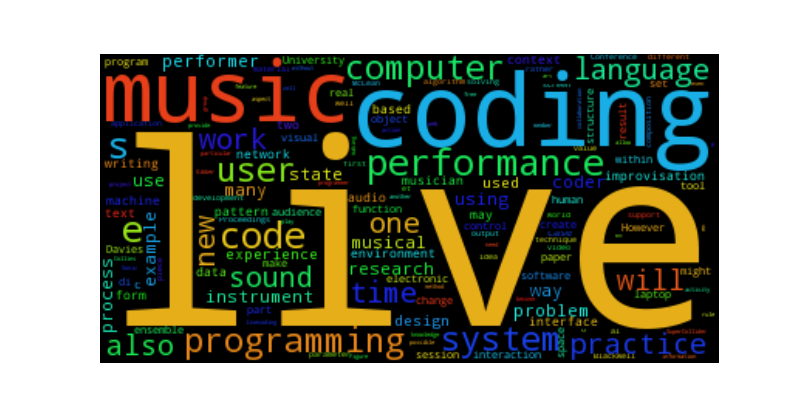
\includegraphics[scale=0.71]{./imagens/livecoding_cloud1.png}
\caption{Nuvem de palavras dos anais ICLC2015 \textbf{Fonte}: autor.}
\label{fig:nuvemlivecoding}
\end{center}
\end{figure}

\begin{table}
\caption{Tabela de classes qualitativas de termos utilizados nos anais do ICLC2015, agrupados por funções textuais.}
\small
    \begin{tabular}{ p{1.6cm} | p{1.4cm} | p{2cm} | p{1.45cm} | p{1.45cm} | p{1.45cm} | p{1.45cm} | p{1.45cm} | p{1.2cm}}
    \hline 
    \hline 

    \tiny \textbf{Número Qualitativo/Função} & \textbf{0} & \textbf{1}  & \textbf{2} & \textbf{3} & \textbf{4}  & \textbf{5} & \textbf{8} & \textbf{9}\\
    \hline 
    \hline 

    \tiny \textbf{Pessoas}  
    & - 
    & \tiny Collins, Blackwell, McLean, Grossi 
    & - 
    & - 
    & - 
    & -  
    & - 
    & - \\
    \hline

    \tiny \textbf{Aplicativos}
    & - 
    & \tiny SuperCollider, Gibber, SonicPi  
    & - 
    & - 
    & - 
    & -  
    & - 
    & \\
    \hline
    
    \tiny \textbf{Verbos}  
    & \tiny take, see, shared, networked, explore, made
    & \tiny make, provide, writing, solving, making
    & \tiny used
    & \tiny using, coding  
    & \tiny performer
    & - 
    & - 
    & -  \\
  \hline

     \tiny \textbf{Adjetivo ou numeral, ordinal}  
    & \tiny less, open, potential, similar, important, cognitive, virtual
    & \tiny first, real, electronic, visual, ensemble, possible, free, livecoding, aspect  
    & \tiny musical, many
    & \tiny new, one
    & - 
    & -  
    & \tiny live 
    & - \\
    \hline

    \tiny \textbf{Substantivo}  
    & \tiny Browser, point, approach, order, node, collaborative, number, source, present, community, server, framework, orchestra, digital, level, kind, type, memory, analysis, line, body, concept, technology, working, org, current, show, mean, end, processes, people, international
    & \tiny University, conference, proceedings, network, interface, environment, text, form, context, musician, space, paper, program, audience, function, change, control, human, laptop, interaction, structure, part, session, tool, result, create, object, case, algorithm, value, development, material, set, technique, parameter, idea, screen, video, application, support, composition, piece, knowledge, feature, cell, activity, art, action, information, method, web, rule, group, need, particular, project, allow, collaboration, programmer, member, play, output 
    & \tiny use, coder, process, state, example, way, software, research, problem, experience, design, improvisation, different, machine, pattern, audio
    & \tiny work, instrument
    & \tiny system, computer, user, language, time, practice, sound
    & \tiny programming
    & \tiny performance, code
    & \tiny ``live coding'', music  \\
    \hline
    \hline
   
    \end{tabular}
\label{tab:comparacao}
\end{table}

Uma breve análise da nuvem de palavras pode elucidar parte das questões-satélites. Na \autoref{tab:comparacao} filtrei parte dos resultados na nuvem de palavras por conjuntos de funções textuais -- sujeitos-humanos, sujeitos-ferramentas, verbos, adjetivos e substantivos -- e quantas vezes foram utilizados, em categorias qualitativas (0, menos usado e 9 o mais usado, sendo que 6 e 7 não apresentaram resultados). \footnote{O método de extração será explicado em um apêndice oportuno.}. 

No caso dos sujeitos-humanos, podemos ver nomes de Nick Collins e Alex McLean, praticantes responsáveis pela criação de um manifesto, cujo um fragmento será discutido no capítulo 2. Pietro Grossi, é um personagem recentemente estudado por \citeonline{mori_pietro_2015} como um caso prematuro de \emph{live coding}, a partir do final da década de sessenta.

No caso dos sujeitos-ferramentas, destacamos o papel do \emph{SuperCollider}, já citado anteiormente, e do \emph{Gibber}\footnote{Disponível em \url{http://gibber.mat.ucsb.edu}}. Ambos são ambiente de programação para de síntese sonora e composição algorítmica. Uma semelhança paradigmática para estes ambientes, é o procedimento de compilação de códigos conhecido como \emph{Just In Time} \cite{aycock_brief_2003}. Enquanto no primeiro \emph{software} a questão está posta em uma máquina -- \emph{laptop} -- local, o \emph{Gibber} representa a viabilidade do navegador de \emph{internet} como plataforma musical \citeonline{roberts_gibber:_2012,wyse_viability_2014}.

Os verbos fornecem informação sobre o comportamento dos improvisadores de códigos. Além da atividades como \emph{performatizar} e \emph{codificar}, é notável atividades sociais ligadas à visão, à escrita, à técnica, à lógica. Embora a Música seja a atividade proeminente do \emph{live coding}, não obtivemos resultados que retornassem, por exemplo, a palavra \emph{hearing}. Isso é significativo, e no \autoref{cap:trabalhos_relacionados}, exploro estas ações sob a ótica da Música de Processos de Steve Reich.

Já os adjetivos destacam características da prática, onde \emph{live} é a palavra-chave. Como será observado no \autoref{cap:trabalhos_relacionados}, a ação pode ocorrer em uma sala de concerto, um espaço público ou em uma casa noturna. Palavras como  \emph{electronic}, podem sugerir tanto uma música ``eletroacústica'', quanto gêneros de música para dançar. \emph{Visual} remete a uma característica tão fundamental quanto a Música. Um sem número de performances utilizam a projeção de telas de computadores como dispositivo de ``transparência''; isto é, uma ideologia de justificação do ato de improvisação. \emph{Ensemble} destaca uma a natureza de grupos. Poucas performances \emph{solo} são realizadas se comparadas às performances de \emph{duos}, \emph{trios}. 

Substantivos relacionam a atividade como processo (\emph{process}). Como será discutido no Capítulo 2, o \emph{live coding} se apropria de conceitos da Música como Processo de Steve Reich e da Música Generativa de Brian Eno para justificar um processo de codificação incessante. Por outro lado, palavras como \emph{university}, \emph{research} e \emph{technology}, e \emph{laptop} acusam não apenas uma prática artística, mas um programa de pesquisa tipo de performance, que utiliza um computador para resultados audiovisuais, realizados por universitários. A esfera de pesquisa acadêmica permitiu ramos de desenvolvimento com linguagens de programação, cognição, inteligência artificial, semiologia, performance musical (improvisação), e mais recentemente, etnologia, conferindo à produção de \emph{live coding} uma aura de legitimidade escolar.